\chapter{Behavioral Cloning for Autonomous Driving through the Obstacle Course}
\label{cha:Main}

\section{Environment Setup}

\subsection{Arena}

The arena used in this thesis is represented as a \(2 \times 1\) meter surface, on which obstacles measuring \(4 \times 4 \times 16\) cm are placed. The setup resembles the one used in König’s thesis \autocite{konig2022model}, with the key difference being that all obstacles in the current thesis are of a single color. To ensure measurement precision as well as material stability and robustness, 3D-printing technology was chosen for obstacle fabrication. This approach also facilitates a smooth transition to virtual reality, in case virtualization becomes necessary.

To address the first difficulty, the obstacles were glued to the arena surface to ensure they maintained their exact positions during preparation and evaluation. However, for the second difficulty (where frequent repositioning of obstacles is required) they were left unglued. In each experimental run, three pairs of obstacles are installed on the arena. Their positions are deliberately selected to maximize the likelihood that they remain within the camera’s field of view until the robot passes them.

\subsection{Hardware}

To collect training data and evaluate the trained models, the NVIDIA JetBot is employed, consistent with previous research conducted by ScaDS.AI. The JetBot is powered by a Jetson Nano module, which features 4 GB of LPDDR4 memory and 128 CUDA cores, capable of running at a maximum clock speed of 921 MHz. These computational capabilities are sufficient to execute the entire control inference pipeline at a frequency of 4 Hz, ensuring timely responses for real-time navigation tasks. The detailed description of the pipeline is represented in \autoref{sec:pipeline}.

The movement system consists of two DC motors with integrated encoders, connected to the Jetson Nano through a motor driver interface. This allows the control of the robot’s differential drive mechanism, enabling it to perform turns and controlled straight motion. The motors are powered by a rechargeable lithium-ion battery, providing enough energy for several hours of operation under typical loads.

For motor control and overall robot management, the JetBot API was used, which conveniently provides \texttt{Python} bindings. This allows integration with the data acquisition and inference components, all of which are written in \texttt{Python}. Although the API includes various methods to control the JetBot, this thesis adopts the direct velocity control method. For each of the two motors the velocity can be set to any value within the range \([-1, 1]\), where \(-1\) corresponds to full reverse, \(0\) to a stationary motor, and \(1\) to full forward speed. This approach simplifies the control logic and makes the task of mapping the joystick inputs to control signals more straightforward.

Additional peripherals include a wide-angle Raspberry Pi Camera BMP (V2) module, used for visual input, and a Wi-Fi module for remote access and debugging. The camera captures frames at a resolution suitable for both training and real-time inference with the maximum frame rate of 120 Hz.

\subsection{Software}

To facilitate frequent modifications to the model architecture, the \texttt{Keras} framework was chosen for development. \texttt{Keras} is a high-level neural network API for \texttt{Python} programming language built on top of \texttt{TensorFlow}, which handles GPU acceleration, memory management, and other low-level operations. This abstraction significantly simplifies the design and training of deep learning models. The primary motivations for selecting \texttt{Keras} include its intuitive syntax, extensive library of pre-built layers, activation functions, loss functions, and optimizers, as well as its strong community support and documentation.

\texttt{Keras} also includes a convenient toolkit for training workflows, featuring integrated support for image data preprocessing and augmentation. However, since this thesis involves working with temporal sequences of image frames, which requires accurate frame rate consistency for the training, a custom data augmentation pipeline was implemented. This custom solution ensures that temporal integrity is maintained when transforming image sequences during training, which is critical for models that rely on time-dependent input data.

During development, version compatibility issues were encountered, particularly with \texttt{TensorFlow} on the Jetson Nano hardware. The Jetson platform supports only specific versions of cuDNN, a prerequisite for GPU-accelerated \texttt{TensorFlow}. Consequently, it was necessary to downgrade \texttt{TensorFlow} to a compatible version across the entire project to maintain consistency between training and experimental environments.

For numerical operations, the \texttt{NumPy} library was employed. \texttt{NumPy} provides a rich collection of mathematical functions that are implemented in optimized \texttt{C/C++} code. This enables efficient numerical computation in \texttt{Python}, which is essential for tasks such as preprocessing datasets, manipulating input tensors, and analyzing model outputs.

All image processing tasks, including resizing, cropping, filtering, and saving frames, were performed using the \texttt{OpenCV} library. \texttt{OpenCV} offers an extensive suite of image manipulation functions and is highly optimized for real-time performance. It proved indispensable throughout the development process, particularly during data collection, visualization, and debugging phases.

\section{Data Acquisition}

To perform supervised learning using Behavioral Cloning, it was necessary to collect a labeled dataset. The dataset \( D \) is represented as a sequence of input-output pairs \( (x_i, y_i) \in D \), where \( x_i \) denotes the sensor input (in this case, camera frames), and \( y_i \) represents the corresponding control signal required for the robot at that point in time. To generate these labels, a gamepad was used, with the inclination of its left analog stick mapped to motor speed values for the JetBot using a special function.

To streamline the data collection process, a custom data acquisition pipeline was developed. Its primary goals were to (1) allow real-time control of the JetBot via the gamepad, (2) capture synchronized sensor data, and (3) store the collected data in a structured format. The pipeline consists of two components:

\begin{itemize}
  \item \textbf{Server}: runs on the JetBot and handles both motor control and video capture.
  \item \textbf{Client}: runs on an external machine connected to the same local network, responsible for reading gamepad inputs and sending them to the server.
\end{itemize}

The pipeline operates as follows:

\begin{enumerate}
  \item The server program is launched on the JetBot. It spawns two concurrent threads:
    \begin{itemize}
      \item One thread initializes the OpenCV video capture pipeline to continuously collect frames from the onboard camera.
      \item The second thread starts a TCP server using \texttt{Python}’s built-in \texttt{socket} library, listening for incoming connections on a designated port.
    \end{itemize}

  \item The client program is executed on another machine. It verifies the presence of a connected gamepad and begins listening for control inputs using the \texttt{pygame} library, which provides low-level access to hardware devices.

  \item Once a connection is established, the client begins transmitting the current position of the gamepad’s left analog stick to the JetBot server.

  \item The TCP server thread on the JetBot receives the input data and updates a shared variable, which is accessed by the video thread.

  \item When a new video frame is captured, it is stored locally. Simultaneously, the server retrieves the most recent gamepad input from the shared variable and calculates the corresponding motor speeds. For an analog stick input represented as \( (x, y) \), the left and right motor speeds are derived using the calculations described in Algorithm \ref{alg:motor_inputs}.

  \item The computed motor commands are then sent to the JetBot’s motors via the JetBot API, and the process repeats in real time until manual termination.

  \item Upon termination, the collected data is transferred from the JetBot to the client machine. All captured video frames are stored in a dedicated directory as image files, while the control sequence is saved in the same directory using NumPy's binary format (\texttt{.npy}). Each control entry is stored as a tuple \( (x, y, t) \), where \( x \) and \( y \) are the analog stick positions, and \( t \) is the timestamp in milliseconds from the start of the recording session.
\end{enumerate}

\begin{algorithm}
  \caption{Calculation of motor inputs based on the gamepad's stick position}
  \begin{algorithmic}[1]
    \Function{CalculateMotorInputs}{$x, y$}
    \State $\text{rotation\_quotient} \gets 0.5$
    \State $left\_power \gets -y + x \cdot \text{rotation\_quotient}$
    \State $right\_power \gets -y - x \cdot \text{rotation\_quotient}$
    \State $max\_power \gets \max\left( \left|left\_power\right|, \left|right\_power\right|, 1 \right)$
    \State $left\_power \gets left\_power / max\_power$
    \State $right\_power \gets right\_power / max\_power$
    \State \Return $left\_power, right\_power$
    \EndFunction
  \end{algorithmic}
  \label{alg:motor_inputs}
\end{algorithm}

The data was initially collected at a frame rate of 30 frames per second (FPS). However, it was later decided to increase the frame rate to 120 FPS, as it is the fastest framerate that the sensor can provide. The rationale behind this decision was that, although the system is not capable of executing the control policy at such a high frequency in real-time, the high-frame-rate sequences could be downsampled during training using time and frequency warping techniques \autocite{iglesias2023data}. This allows for greater flexibility in choosing the effective temporal resolution for training, depending on the model architecture and experimental requirements.

After data collection, a filtering step was applied to remove unrepresentative or low-quality trajectories. In particular, sequences that did not contribute meaningful information to the learning process (such as those recorded after the JetBot had passed the final obstacle pair) were discarded entirely. Additionally, some valid trajectories were cropped to eliminate irrelevant frames that might hinder effective feature extraction during training.

The final dataset consists of 22,017 labeled images and is divided into two subsets: one for the first difficulty level and the other for the second difficulty level. The first difficulty subset contains 15,008 data points, while the remaining 7,009 correspond to the second difficulty.

It is important to note that the quality and quantity of data for the second difficulty level are suboptimal. Compared to the first difficulty, the second requires a significantly higher degree of generalization from the model due to increased environmental variability. Ideally, the dataset for the second difficulty would have included more examples with greater diversity and a broader distribution of features. However, due to time constraints, the substantial workload involved in completing this thesis, and the labor-intensive nature of data acquisition and filtering, it was decided to proceed with training using the existing dataset.

\section{Data Pre-processing}

Before initiating the training process, the collected data must be pre-processed to enhance training efficiency and reduce the impact of irrelevant noise that could impair the model's ability to learn meaningful features. The pre-processing steps applied to the images and used in the final training iteration are illustrated in \autoref{fig:preprocessing} and outlined below:

\begin{enumerate}
  \item \textbf{Grayscale Conversion} \\
    Due to hardware limitations in terms of memory and computational resources on the JetBot platform, the model must be lightweight and capable of making inferences in real time. To reduce computational complexity and model size, all images are converted to grayscale prior to being fed into the neural network. This eliminates color information while preserving structural features necessary for decision-making. The grayscale transformation is performed using the standard luminance-preserving formula:
    \[
      Y = 0.299 \times R + 0.587 \times G + 0.114 \times B
    \]
    where \( R \), \( G \), and \( B \) denote the red, green, and blue color channels, respectively.

  \item \textbf{Region of Interest (ROI) Cropping} \\
    To further reduce the computational load and focus the model’s attention on the most relevant parts of the input, a region of interest is cropped from each image. This not only reduces the input dimensionality (thereby speeding up both training and inference), but also increases the proportion of informative pixels that are likely to contribute to effective feature extraction.

  \item \textbf{Pixel Centering} \\
    Convolutional Neural Networks (CNNs) typically benefit from normalized input data. As shown in prior research \autocite{pal2016preprocessing}, normalization helps accelerate convergence and improve model performance. In the final model implementation, all grayscale images are centered around zero by applying the following normalization:
    \[
      Y_c = \frac{Y}{127.5} - 1
    \]
    where \( Y \) is the grayscale image matrix and \( Y_c \) is the normalized output passed to the network.

    Z-score normalization approach was also experimented on, but it didn't show any better results compared to the pixel-centered approach.

  \item \textbf{Update memory stack} \\
    Once the image is passed through all of the preprocessing steps, the memory stack of size $N$ is updated by pushing the frame to its top position. The stack size $N$ is usually set to $10$ after hyperparameter tuning that yielded the best parameters with which the model has the best training results.
\end{enumerate}

\begin{figure}[htbp]
  \centering
  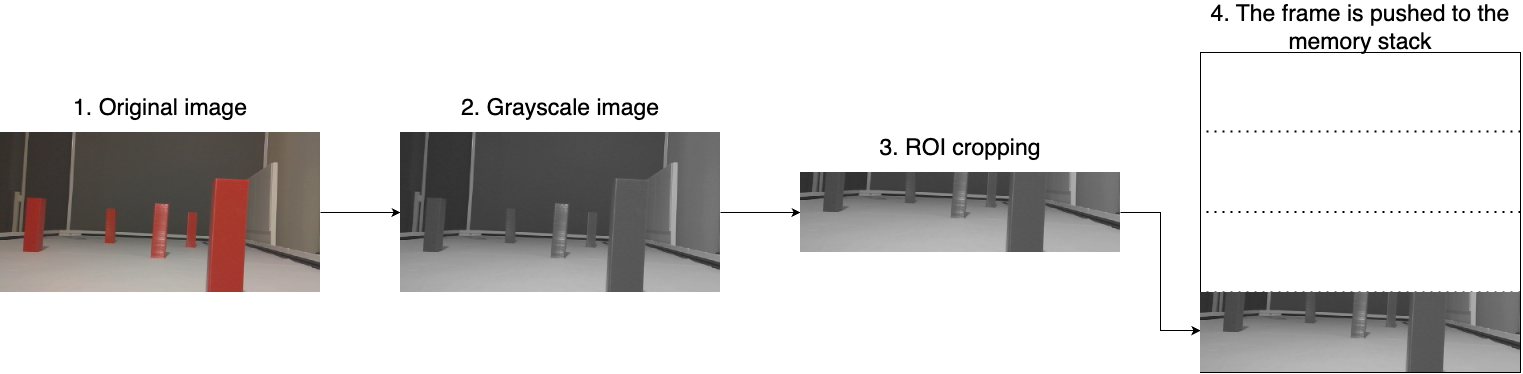
\includegraphics[width=0.9\textwidth]{Images/preprocessing.png}
  \caption{Input preprocessing pipeline.}
  \label{fig:preprocessing}
\end{figure}

\subsection{Edge Detection}
\label{sec:edge-detection}

Although the final version of the agent utilizes relatively simple and direct pre-processing steps, a substantial amount of experimentation was conducted to evaluate other more advanced techniques and determine the most effective configuration.

One such technique, proposed as a direction for future work by Farag et al. \autocite{8855753}, is the application of edge detection to input images prior to processing by a Convolutional Neural Network (CNN). The intuition behind this method is that edge detection enhances object boundaries, potentially making it easier for a CNN to extract meaningful features from the input. This, in theory, could simplify the task of identifying obstacles and accelerate the model’s ability to learn complex and task-relevant visual patterns.

To test this hypothesis, two well-known edge detection algorithms were evaluated: the Canny edge detector \autocite{canny1986computational}, as recommended by Farag et al. \autocite{8855753}, and the Sobel filter \autocite{sobel2014history}. These approaches were selected, because after testing multiple edge detection algorithms, they seemed to produce the most meaningful and noiseless outputs. Models were trained using data processed by each of these algorithms. However, empirical results showed no significant improvements in performance or generalization capability. The best outcome achieved with edge-detected inputs was that the JetBot was able to consistently pass the second pair of obstacles but failed to navigate the third.

\begin{figure}[htbp]
  \centering
  \tabulinesep=1.2mm
  \begin{tabu}{cc}
    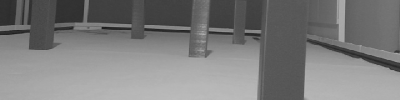
\includegraphics[width=0.4\textwidth]{Images/EdgeDetection/original.png} & 
\includegraphics[width=0.4\textwidth]{Images/EdgeDetection/blurred.png} \\
    \parbox{0.4\textwidth}{\centering (a) Original grayscale image.} &
    \parbox{0.4\textwidth}{\centering (b) Gaussian Blur is used to remove the noise before applying edge detection.} \\
    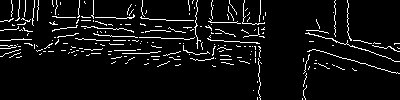
\includegraphics[width=0.4\textwidth]{Images/EdgeDetection/canny_edges.png} & 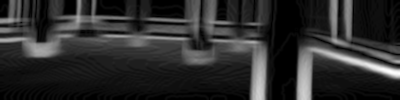
\includegraphics[width=0.4\textwidth]{Images/EdgeDetection/sobel_edges.png} \\
    \parbox{0.4\textwidth}{\centering (c) Canny edge detection algorithm.} &
    \parbox{0.4\textwidth}{\centering (d) Sobel filter applied to the image in $x$ and $y$ directions.} \\
    
\includegraphics[width=0.4\textwidth]{Images/EdgeDetection/morphological_edges.png} & 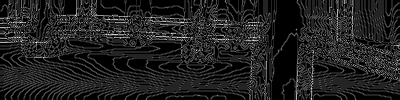
\includegraphics[width=0.4\textwidth]{Images/EdgeDetection/log_edges.png} \\
    \parbox{0.4\textwidth}{\centering (e) Morphological gradient operation for edge enhancement.} &
    \parbox{0.4\textwidth}{\centering (f) Laplacian of Gaussian (LoG) edge detection.} \\
  \end{tabu}
  \caption{Examples of the output of different edge detection algorithms.}
\end{figure}

In contrast, the baseline model trained on unprocessed grayscale images exhibited significantly better performance. The poor results with edge-detected inputs are likely due to the sensitivity of these algorithms to noise. Although Gaussian blurring was applied to smooth the images and reduce noise, both Canny and Sobel methods still introduced visual artifacts that the model may have incorrectly interpreted as important features.

While edge detection remains a conceptually promising technique, it did not yield practical benefits in the context of this project. An additional idea explored was the use of Quantized Neural Networks (QNNs), in which network weights are represented as low-precision integers or even binary values. Given that the Canny edge detector produces binary output, it would be theoretically feasible to design a quantized CNN specifically tailored to such input. This approach could significantly reduce model size and enhance computational efficiency, as integer operations are less resource-intensive than floating-point calculations. However, due to time constraints and the lack of observed performance gains from edge detection, this prospect was not pursued further in this work.

\section{Model Architecture}

One of the primary objectives of this thesis was to design a Convolutional Neural Network (CNN) architecture capable of effectively learning and extracting relevant features from image sequences. As in previous works, the model would need to capture not only spatial features from individual frames but also temporal dependencies across a sequence of images. This requirement necessitated the incorporation of a memory mechanism, as introduced in prior works such as \autocite{schneeberger2024end} and \autocite{schaller2023train}.

To identify the most suitable model architecture for the task, various configurations and design strategies were explored. Dozens of architectures were implemented and evaluated, with many discarded early due to poor performance. Below is a summary of some of the architectures that were tested on the way of reaching the satisfactory results:

\begin{enumerate}
  \item \textbf{Previous Thesis-Based Approach:} \\
    The architectures proposed by Schneeberger \autocite{schneeberger2024end} and Schaller \autocite{schaller2023train} processed the input image sequence using multiple convolutional channels --- one per image. To replicate this design, the CNN model from OpenAI’s Stable Baselines 3, originally implemented in \texttt{PyTorch}, was reimplemented in \texttt{Keras} and adjusted to conform to dimensional requirements. The architectural layout is shown in \autoref{fig:sb3cnn-arch}.

    \begin{figure}[htbp]
      \centering
      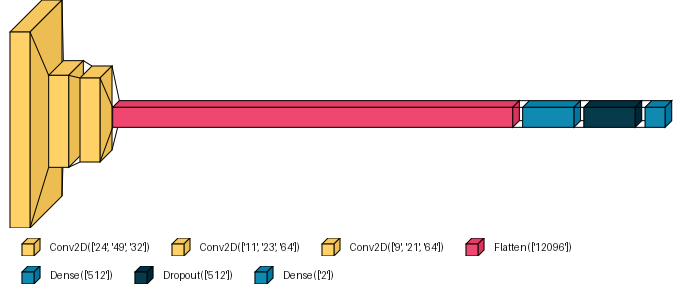
\includegraphics[width=0.8\textwidth]{Images/SB3CNN_architecture.png}
      \caption{Architecture diagram of the CNN model from Stable Baselines 3.}
      \label{fig:sb3cnn-arch}
    \end{figure}

    This model didn't show the ability to learn from the given dataset, most likely due to it being too shallow to be able to capture meaningful features from high-dimensional inputs. The validation loss sank early, causing the Early Stopping mechanism to terminate training at epoch 10.

  \item \textbf{DAVE-2:} \\
    This architecture, originally developed by NVIDIA researchers \autocite{bojarski2016endendlearningselfdriving}, was replicated exactly as described in the original publication. It is the only model evaluated in this thesis that does not incorporate any memory mechanism and also does not require preprocessing beyond simple image cropping. The network accepts raw RGB images as input using a 3-channel input layer and is visualized in \autoref{fig:dave-2-arch}.

    \begin{figure}[htbp]
      \centering
      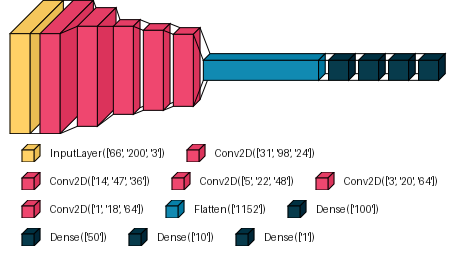
\includegraphics[width=0.5\textwidth]{Images/DAVE-2_architecture.png}
      \caption{DAVE-2 architecture.}
      \label{fig:dave-2-arch}
    \end{figure}

  \item \textbf{BCNet with LSTM:} \\
    BCNet, proposed by Farag et al. \autocite{8855753}, shares structural similarities with DAVE-2 but includes key differences such as the number and sizes of layers. While originally designed to predict the vehicle’s steering angle, the model was adapted for this thesis to conform to the task of predicting the velocity of the motors.

    In their work, Farag et al. also proposed several potential improvements, including the integration of Long Short-Term Memory (LSTM) layers and the use of edge detection during preprocessing. As discussed in \autoref{sec:edge-detection}, edge detection did not yield beneficial results in this context. However, the integration of LSTM layers was implemented to capture temporal patterns in the image sequence.

    Both LSTM and convolutional LSTM layers were planned to be experimented on. However, since the \texttt{cuDNN} version installed on the JetBot is not the latest, some CUDA API features that are required to use \texttt{Keras}’s \texttt{ConvLSTM2D} with GPU acceleration are not available. For this reason only casual convolutional LSTM layers were utilized to implement the architecture design of the model.

    The resulting architecture is illustrated in \autoref{fig:BCNet-LSTM-arch}. To integrate the LSTM component, \texttt{Keras}’s \texttt{TimeDistributed} layers were employed. These layers apply convolutional operations to each frame in the sequence independently, enabling the sequential outputs to be passed collectively to the LSTM block for temporal processing.

    \begin{figure}[htbp]
      \centering
      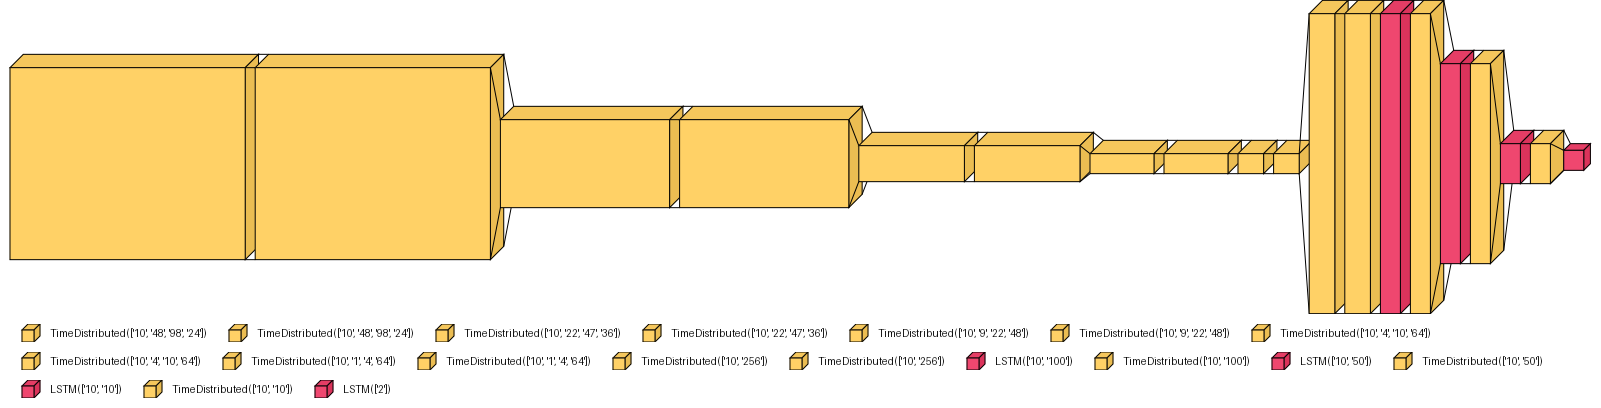
\includegraphics[width=1.0\textwidth]{Images/BCNetLSTM_architecture.png}
      \caption{BCNet with LSTM layers. The \texttt{TimeDistributed} layers represent convolutional, flattening, and dropout operations across the sequence.}
      \label{fig:BCNet-LSTM-arch}
    \end{figure}
\end{enumerate}

\section{Training Process}

The training process for the models involves multiple stages, including data preprocessing, dynamic batching, augmentation, and iterative refinement of model hyperparameters. Due to the constraints of hardware resources, the training pipeline must be both efficient and robust. One of the main components enabling this is the data generator, which is responsible for assembling input sequences and labels on the fly, thereby allowing for large-scale training without exceeding system memory limits.

\subsection{Data Generator}

Given the size of the dataset, which exceeds the available Random Access Memory (RAM) on most devices, a dynamic data generator is implemented. Its primary function is to generate training data sequences incrementally, processing and yielding data batch by batch during training.

The generator constructs temporal sequences of input frames, ensuring that the interval between consecutive frames in each sequence is not shorter than the minimum time interval required by the control inference pipeline to operate effectively. This interval is determined based on timestamp differences stored in the dataset. If a particular frame is the first in a trajectory and lacks any predecessors, the memory stack is padded with zero-valued matrices to account for the missing historical context.

For training, a maximum frame frequency of 4 Hz is typically used. This rate provides a balance between temporal resolution and computational load and is sufficient for most models to make their predictions, particularly when controlling the JetBot at low velocities.

After all frames are pre-processed and collected into the memory stack, a corresponding label must be generated for the data sequence. The label is obtained from the coordinates of the joystick's left analog stick in the frame immediately following the last frame in the sequence. Several alternative strategies were explored, including predicting the joystick position of the current frame or of a frame two steps ahead. However, predicting the next frame's joystick position yielded the best results. This can be explained by the latency of the inference pipeline: the system requires approximately $\frac{1}{4}$ seconds to compute the motor commands and invoke the API to apply them. In the case the model requires less time for the prediction, the pipeline is artificially slowed down to conform the target frequency. By the time this process is complete, the system's state has already changed. Therefore, predicting the immediate future state (i.e., the next frame) aligns more closely with real-world control requirements.

An alternative approach was also evaluated, where the labels consisted of direct motor velocity signals rather than joystick coordinates. This method is inspired by the research of Hwangbo et al. \autocite{hwangbo2019learning}, who reported improved performance when training legged robots using low-level actuator signals. However, in experiments run on the JetBot, using motor velocities as labels led to significantly worse model performance compared to using analog stick coordinates. This difference is likely due to differences in robot construction (legged vs. wheeled), training methodologies, and experimental setups.

Once the state-label pair is assembled, it is stored in a buffer array used for data augmentation. The number of stored instances is determined by a user-defined parameter passed to the data generator. During subsequent iterations, with a certain probability, the generator may retrieve a stored pair from the augmentation buffer, apply a set of transformations (see \autoref{sec:augmentation}), and yield the augmented data before proceeding with the next unmodified pair.

If the data generator completes an iteration over all data points within a given subset of the dataset and entries remain in the augmentation buffer, it proceeds to process each of these stored entries. This stochastic sampling logic ensures that transformed pairs are not immediately following their original counterparts. Moreover, this approach guarantees that each data point is replicated and transformed precisely the number of times specified by the user-defined augmentation parameter.

The step-by-step description of the data generator is described in the Algorithm \ref{alg:data_generator}.

\subsection{Data Augmentation}
\label{sec:augmentation}

Data augmentation is a well-established strategy for improving model generalization, especially in cases where collecting large, diverse datasets is infeasible. In the context of time series data, augmentation methods can be particularly impactful, since transformations applied by them can modify not only spatial, but also temporal structures of the data \autocite{iglesias2023data}.

This work adopts a hybrid augmentation strategy that applies both temporal and spacial transformations to the training data. For the temporal component, \textbf{time warping} is implemented by dynamically adjusting the maximum allowed frame frequency \( f_{\text{max}} \) for data pairs retrieved from the augmentation buffer. By increasing or decreasing the time between frames in a sequence, the generator effectively simulates variations in system response time or actuation speed, thus improving the model's robustness to timing deviations.

Spacial transformations are also applied to the augmented input data. They're applied probabilistically and independently to each image in the memory stack:

\begin{itemize}
  \item \textbf{Gaussian Noise Injection (Jittering):} Gaussian noise with a random standard deviation \( \sigma \in [0, 0.5] \) is added to simulate sensor noise or varying lighting conditions.
  \item \textbf{Translation:} The image is randomly shifted along both axes within a maximum offset of 9 pixels, simulating minor misalignments or camera movement.
  \item \textbf{Rotation and Scaling:} A small random rotation (up to \( \pm 5^\circ \)) and scaling (within \( \pm 6\% \)) are applied using affine transformations. This accounts for slight perspective distortions and variations in camera zoom.
\end{itemize}

The augmentation process is applied during data generation, immediately before yielding the augmented state-label pair. This ensures that transformations are computed on-the-fly and vary across training epochs, further reducing the risk of overfitting.

By combining time series augmentation principles, as outlined in \autocite{iglesias2023data}, with low-level image manipulation techniques, the data generator enhances both temporal and spacial diversity in the training dataset. This dual-augmentation approach has shown to significantly improve the stability and adaptability of the resulting control model.

\begin{algorithm}[H]
  \caption{Data Generator for Incremental Training with Augmentation}
  \begin{algorithmic}[1]
    \Require Dataset $D$, max frame frequency $f_{max} = 4$ Hz, memory stack size $N$, augmentation factor $k$, augmentation probability $p$
    \Ensure Yields $(state, label)$ pairs for training

    \State Initialize augmentation buffer $A \gets \emptyset$
    \ForAll{data points $d_i \in D$}
    \State Initialize memory stack $M_i \gets \emptyset$
    \State Set current index $j \gets i$
    \While{$|M_i| < N$ and $timestamp(d_j) > 0$}
    \If{$timestamp(d_j) - timestamp(d_{j-1}) \geq \frac{1}{f_{max}}$}
    \State Append $d_j$ to $M_i$
    \EndIf
    \State $j \gets j - 1$
    \EndWhile
    \If{length of $M_i < N$}
    \State Pad $M_i$ with zero-matrices until size $N$
    \EndIf
    \State Extract label $y_i$ from $d_{i+1}$
    \State Store $(M_i, y_i)$ in $A$ $k$ times based on augmentation factor
    \If{random() $< p$ and $A \neq \emptyset$}
    \State Select random $(M_j, y_j)$ from $A$
    \State Apply augmentation to $(M_j, y_j)$ to get $(\hat{M}_j, \hat{y}_j)$
    \State \textbf{yield} $(\hat{M}_j, \hat{y}_j)$
    \EndIf
    \State \textbf{yield} $(M_i, y_i)$
    \EndFor
    \If{$A \neq \emptyset$}
    \ForAll{$(M_j, y_j) \in A$}
    \State Apply augmentation to $(M_j, y_j)$ to get $(\hat{M}_j, \hat{y}_j)$
    \State \textbf{yield} $(\hat{M}_j, \hat{y}_j)$
    \EndFor
    \EndIf
  \end{algorithmic}
  \label{alg:data_generator}
\end{algorithm}

\subsection{Training Setup}
\label{sec:trainingsetup}

The training process was carefully configured using a set of well-established deep learning practices to ensure efficient convergence, prevent overfitting, and promote generalization across unseen data.

\paragraph{Optimizer and Loss Function.}
The model was trained using the Adam optimizer \autocite{kingma2015adam}, a widely adopted method in deep learning due to its ability to adaptively adjust learning rates for each parameter. The objective function minimized during training was the Mean Squared Error (MSE), selected for its suitability in regression tasks, particularly when predicting continuous joystick values within a bounded range.

\paragraph{Activation Functions.}
For the convolutional layers, the Rectified Linear Unit (ReLU) activation function was used. ReLU is known for its simplicity, non-saturating gradient behavior, and computational efficiency. It has also been shown to facilitate the training of deep networks by addressing the vanishing gradient problem \autocite{DBLP:journals/corr/abs-1803-08375}. For the LSTM layer, the hyperbolic tangent (tanh) activation function was employed. This choice is rooted both in theoretical considerations (tanh is the standard activation function used within LSTM cells \autocite{K20222637}) and practical ones, as the model output is expected to lie within the \([-1, 1]\) range, which tanh naturally supports.

\paragraph{Weight Initialization.}
Proper weight initialization plays a crucial role in achieving stable and fast convergence in deep networks. The weights of the convolutional layers were initialized using He initialization \autocite{he2015delving}, which is specifically designed for layers with ReLU activation. For the LSTM layers, Glorot initialization \autocite{glorot2010understanding} was applied, as it balances the variance of activations between layers and is generally well-suited for networks using tanh activations.

\paragraph{Overfitting prophilaxis.}
To mitigate overfitting and improve generalization, $L_2$ \autocite{kukačka2017regularizationdeeplearningtaxonomy} regularization was applied to all trainable layers in the network. In addition, \texttt{EarlyStopping} and \texttt{ReduceLROnPlateau} callbacks provided by the Keras framework were employed. \texttt{EarlyStopping} halts training when no improvement in validation loss is observed over a specified number of epochs, while \texttt{ReduceLROnPlateau} adaptively lowers the learning rate when validation performance plateaus, thus allowing finer convergence without overshooting minima.

\subsection{Hyperparameters}
\label{sec:hyperparameters}

After the identification of the most effective model architecture --- BCNet with LSTM layers (\autoref{fig:BCNet-LSTM-arch}) --- a systematic hyperparameter optimization process was conducted to enhance both training efficiency and experimental performance. For this purpose, the \texttt{Keras Tuner} library was employed. This library offers a scalable and flexible framework for automated hyperparameter search within the \texttt{Keras} framework using strategies such as random search, Hyperband, and Bayesian optimization.

A range of key hyperparameters was explored during the tuning process:

\begin{itemize}
  \item \textbf{Dropout Rates:} Applied to Dropout layers to mitigate overfitting, with values tested in the range \([0.1, 0.7]\).
  \item \textbf{Convolutional Kernel Sizes:} Kernel sizes for convolutional layers were tuned to optimize the balance between feature locality and spatial abstraction.
  \item \textbf{L2 Regularization Factor:} An optimal regularization factor to ensure that the gradient stays within an optimal value range.
  \item \textbf{Learning Rate:} A critical hyperparameter for optimizer performance, tested across a logarithmic scale (e.g., \(10^{-5}\) to \(10^{-2}\)).
  \item \textbf{Augmentation Factor:} Controlled the number of augmented samples stored and reused during training, influencing the degree of regularization and data diversity.
\end{itemize}

Many combinations of hyperparameters were evaluated using validation loss. The tuning process was executed using early stopping and Bayesian optimization to increase the accuracy of the process.

The table below summarizes the final selected hyperparameter values used in the best-performing configuration:

\begin{table}[H]
  \centering
  \begin{tabular}{|l|c|}
    \hline
    \textbf{Hyperparameter} & \textbf{Selected Value} \\
    \hline
    Dropout Rate & $0.3$ \\
    Convolutional Kernel Size & $5$ for the first three layers and $3$ for the rest \\
    L2 Regularization Factor & $10^{-4}$ \\
    Learning Rate & $2.5 * 10^{-4}$ \\
    Augmentation Factor & $3$ \\
    \hline
  \end{tabular}
  \caption{Final hyperparameter values selected using Keras Tuner}
  \label{tab:hyperparameters}
\end{table}

This tuning step significantly improved the convergence behavior and generalization ability of the model, leading to more stable and reliable real-world control performance.

\section{Control Inference Pipeline}
\label{sec:pipeline}

% TODO: remake BCNetLSTM diagram with layer names
